%% Background chapter
%% author Liu Peng

Home networking has been a hot topic for quite a few years. Thanks to the rapid development 
of electronics and computer science, home networking devices are getting more affordable 
and more powerful that people would have at least several multimedia devices that can be 
connected to network.

In this chapter, we give a overview of current solutions to home networking,
compare each solution and describe the problem to solve.

\subsection{Overview}
Early research \cite{link_layer_old} \cite{end_user} \cite{link_layer}
 in home networking area  has been made mainly on how to implement home
 networking infrastructures, like the cable connection, wireless connection,
 optical connection etc. So far, it turns out that IEEE 802.11 protocol stack
 is most successful and most widely deployed home networking infrastructure.

Nowadays, a typical scenario is that a wireless route connected to Ethernet
cable or optical cable from network operator, while other devices connect to
the same local network created by the wireless router. A wireless AP is using
802.11 b/g/n/ac protocol, utilize 2.4 GHz or 5 GHz frequency channels and
provide a 100+ Mbps network connection. This bandwidth is sufficient enough for
transmitting High Definition (1080p) videos.

Different device manufactures choose its preferred multimedia-sharing protocols. The development 
of multimedia-sharing protocols has also experienced a long research period. Since late 1990s, 
UPnP protocol has been developed for home networking usage. At that time, XML is popular and 
widely used by different network applications. UPnP is also designed to make full use of XML. 
UPnP is independent of media and device, and it is running on TCP/IP stack, so it can be easily 
applied to modern network devices. 

In June 2003, Sony established the Digital Living Network Alliance (DLNA), a nonprofit collaborative 
trade organization. The DLNA standard is based on widely used UPnP protocol but it added some 
restrictions on media formats and some compatibility requirements. Device hardware and software 
can be certified by DLNA organization to prove that it should work with other devices that also 
passed this certification.

In 2010, Apple quitted DLNA and developed its own multimedia home networking solution, called 
AirPlay. By adding screen mirroring, authentication and RTP music streaming, Apple tried to make 
a more advanced home network sharing system and create a unique user experience between Apple 
products. It indeed attracts people's interest, and the user experience of Apple's product is 
much better than other similar products in the market. 

Two years later, Wi-Fi alliance released its Miracast technology, and participated in pushing 
new standard in wireless home networking. The Miracast uses Wi-Fi direct technology, so that 
it doesn't require a wireless local network, instead, a peer-to-peer connection is created between 
the sharing and receiving devices. After its releasing, some major software and hardware companies 
soon accept the new standard. Google, for example integrated Miracast support into its Android 
operating system, and provide screen-mirroring feature to other Miracast receivers.

The competition is far from the end, in 2013, Google released a 35-dollar dongle, using its 
Chromecast protocol, Chromecast makes it possible to watch YouTube and Netflix video directly 
on TV with such a device. Laptop and mobile devices with official YouTube App or Chrome browser 
can control the dongle through the local network in home. The home networking
has been pushed to cloud, since YouTube and Netflix content are directly
downloaded from Internet, mobile devices just act as a controller of picking interested contents. 

Almost at the same time, September 2013, Spotify, a new startup music service company has also 
taken part in making its own home networking solution, called Spotify Connect, it provides an 
interface for speakers in home access its huge music database, and directly browse and stream 
using mobile application. Home networking has been pushed towards cloud and Internet.

Since so many companies would like to develop their own devices and even their own protocols. 
The market is a bit mess, devices are not compatible with other devices, users have to buy new 
device to have services from those companies like Netflex and Spotify. There is great need of 
creating some thing that can connect those devices in home and make them work together. 

Streambels project is just created for this need, fill the gap between different protocols and 
connect devices in home networking environment.

\subsection{Available solutions}
\subsubsection[UPnP]{UPnP \footnote{Universal Plug and Play}}
The UPnP device architecture \cite{upnp} \label{upnp} includes seven parts
below:

\begin{enumerate}
\item Addressing \\
UPnP devices have a DHCP client and searches for a DHCP server when connected to the network. 
An UPnP device firstly scans for the DHCP server and then requests an IP address when the DHCP 
server is found. Otherwise, if there is no response from DHCP server, the device uses automatic 
IP address. It randomly chooses an address in the 169.254/16 random and tests it using ARP probe 
to determine if it is already used. The same procedure repeats until an unused address is found. 
After first IP address is set, it then will periodically check for DHCP server, when a server 
responds, it will use the assigned addresses and stop using the address generated by Auto-IP 
after a period of parallel use to complete interactions in progress.
If there is DNS server in the network, it can also use domain names instead of the numerical IP address.
\item Discovery \\
UPnP devices advertise their services to network using UPnP discover protocol, which is based on 
Simple Service Discovery Protocol (SSDP). An UPnP control point also searches the existence of 
UPnP devices in the network using SSDP. The discover message contains a few specific attributes 
of a device and its services, these attributes include device type, unique identifier and a 
pointer to more detailed information.
The device send multicast several NOTIFY message to a pre defined address and port to advertise 
its availability. A control point will listen to this standard multicast address of and get 
notifications when new devices are available in the network.
An advertisement message has its lifetime, so devices in the network will periodically send 
NOTIFY message before the previous message expires. When the device or servers becomes unavailable 
or shut down intentionally, previous advertisements are canceled by sending cancellation messages, 
otherwise, the advertisements will eventually expire on its own.
Control point can search for devices actively by multicasting an SSDP Search message. Other devices 
in the network will respond to the search message by unicasting directly to the requesting control point.
\item Description \\
The discovery message contains URL to the description information. A control point can send HTTP 
GET request to the URL to get detailed UPnP description of the device. The description includes 
a device description and several service descriptions. 

A device description includes vender related information such as model name, serial number and 
manufacture name. A device may have many services, for each service, the device description lists 
the service type, name and URL to the detailed service description, control and eventing. A device 
description may also include embedded devices and a URL to a presentation page.

A service description includes a list of actions that servers can accept, arguments of each action, 
and a list of state variables. The state variables reflect the device's status during runtime.

The description is in XML syntax and is based on standard UPnP device template or service template, 
which is defined by UPnP forum. The template language is written in XML syntax and is derived from 
an XML schema language, so it is machine-readable and automated tools can parse check easily.

By using description, vender has the flexibility to extend services, embed other devices and include 
additional UPnP services, actions or state variables. The control point can be aware of these added 
features by retrieving device's description.
\item Control \\
A control point can ask services in a device to invoke actions by sending control messages. The control 
process is a form of remote procedure call: a control point sends the action to device's service, and 
when the action has completed on the remote device, the service returns the results or errors of the action.

The control messages are expressed in XML using the Simple Object Access Protocol (SOAP) and sent by 
HTTP request. The action results are also received by HTTP responses. The action may cause state variable 
change and those changes will be reflected in the eventing messages.
\item Eventing \\
UPnP service description defines a list of state variables, which updates at runtime. The service 
publishes those changed state variables in the form of event messages, and a control point can 
subscribe to this information.

A control point can subscribe the event notification by sending a subscription message to the 
subscription URL specified in the device description and provides a URL to receive the event messages.

Since there is no mechanism to subscribe to a subset of evented state variables, all subscribed 
control points will receive all event messages regardless of why the state variable changed. 

When the subscription is accepted, the device gives a unique identifier for the subscription and 
the duration of the subscription. The device will also send an initialize event message, which 
includes the names and current values for all evented variables.

The event messages are GENA NOTIFY messages, sent using HTTP with a XML body, which specifies the 
names of one or more state variables and new values of those variables. Once the state variable 
changed, the event message is sent immediately sent to control point, thus the control point can 
get timely information and could display a responsive user interface. The control point then send 
HTTP OK message to acknowledge device that the event message is received. The event message also 
contains a sequence number that allows the detection of possible lost or disordered messages.

The subscription must be renewed periodically to extend lifetime and keep it active. The renew 
message which contains the subscription identifier is sent to the same URL in the subscription 
message. When the subscription expires, the device will stop sending eventing message to the 
control point, and any attempt to renew the expired subscription is rejected.

A subscription can be canceled by sending an appropriate message to the subscription URL.

\item Presentation \\
Many UPnP devices provide a presentation URL to "web" interface for users. User can access the 
presentation URL by a standard web browser. Control point send an HTTP GET request to the 
presentation URL to get a HTML page from the device, and display the page in a web browser, thus 
provide a more user-friendly interface for control and view the status of device. 

The presentation page is totally specified by the device vender, but it must be an HTML page. 
UPnP architecture does not define the details of presentation page, but it should be user friendly 
and have some basic functionality.

\end{enumerate}
\subsubsection[DLNA]{DLNA\footnote{Digital Living Network Alliance}}
DLNA is a pretty old standard in industry compared to other home networking solutions, so it 
is widely used by many manufactures, the newer home networking solution is also influenced by 
DLNA and followed similar technologies. In this paper we focus on the DLNA standard architecture 
so we can have an overview of how a home networking solution will look like.

Three basic functional entities are defined in the UPnP AV architecture: Media Server, Media 
Renderer and Control Point. A physical device can consist of a combination of any of these 
functional entities. A typical example is DLNA Media player is
a combination of a Control Point and a Media renderer.

A simplified DLNA application use scenario\cite{DLNA_proxy} can be seen as
below:

\begin{figure}[htb]
\centering 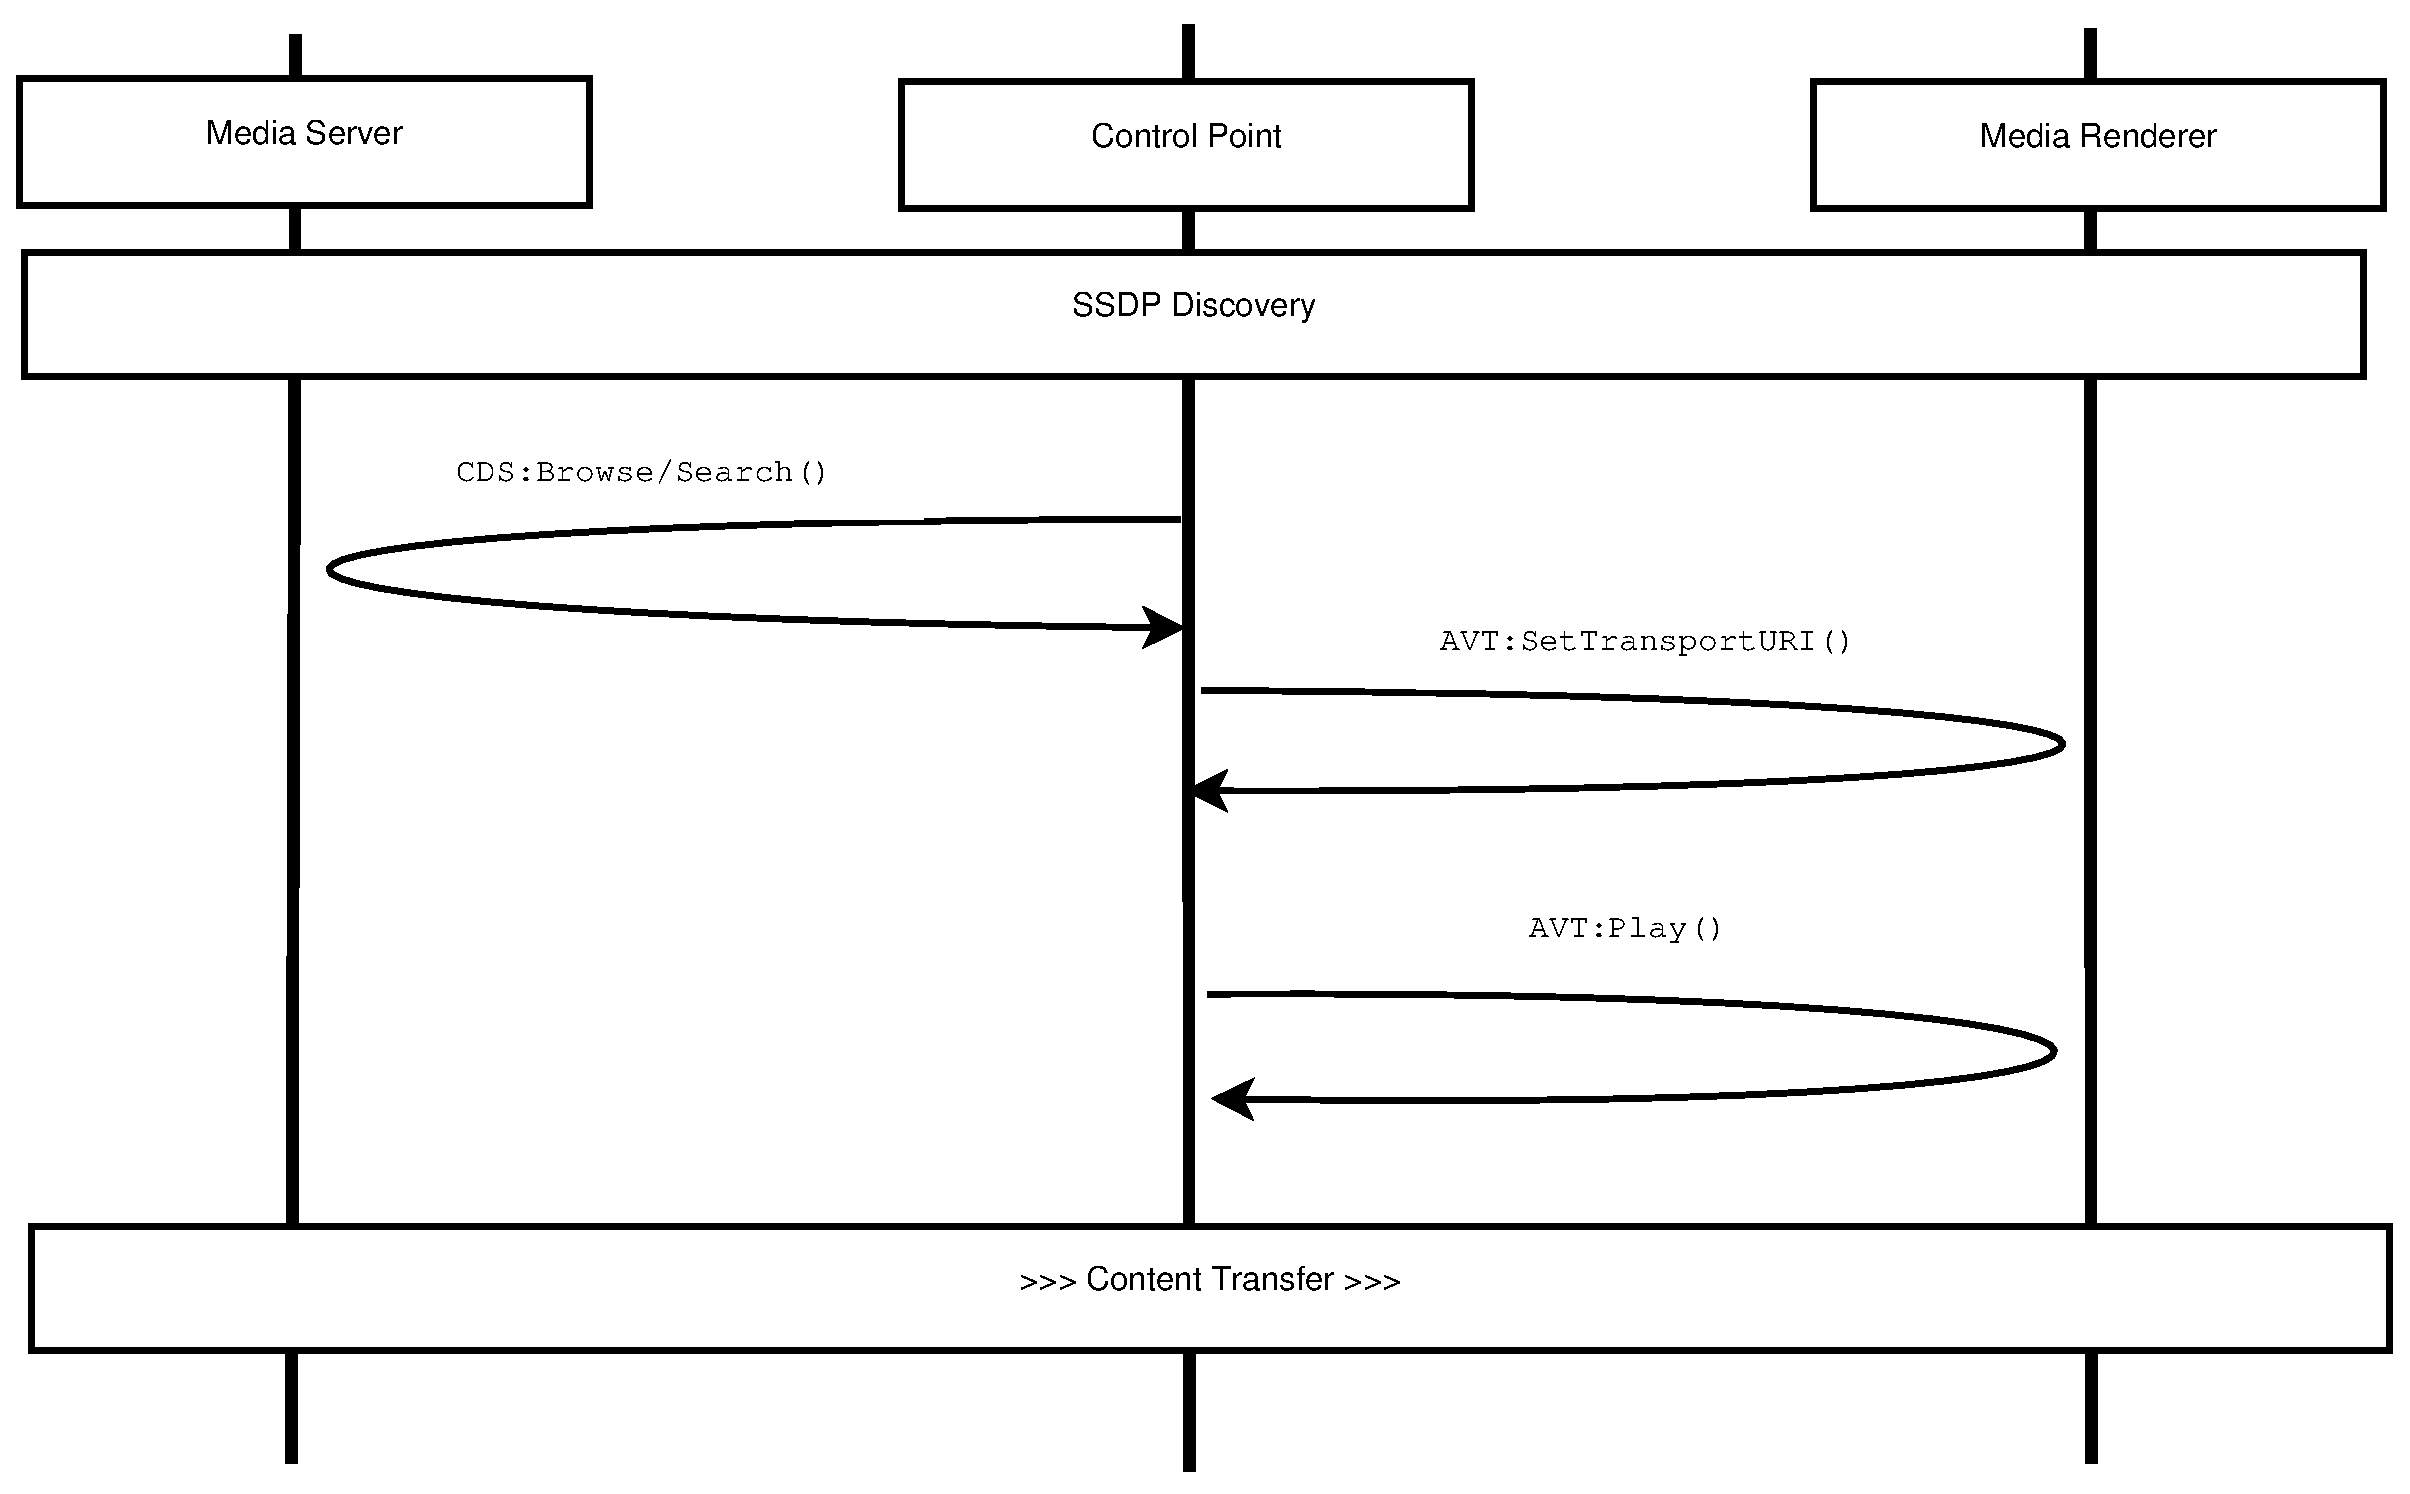
\includegraphics[height=9cm]{charts/chart1}
\caption{DLNA use scenario \label{chart1}}
\end{figure}

The first thing in UPnP network communication is Simple Service Discovery Protocol(SSDP)-based 
device discovery. A SSDP multicast message is send when a new device is added in the network. 
A control point will listen to these multicast messages. When the control point receives the SSDP 
message, the control point sends request for the device's description and services using the location 
provided in the SSDP discovery message. Later the control point can invoke the services action 
command using SOAP.

In media sharing scenario, the control point will browse the information about the Content 
Directory Service (CDS) provided by the Media Server. A browse/Search action can be invoked 
to navigate through the content stored in the Media Server device. When selected the media 
content from Media Server, a Media Renderer AVTransport::SetAVTransportURI will be sent by 
control point to Media Renderer. Finally, the Play command is invoked by control point to 
Media Renderer, and the transfer begin afterwards. The media streaming happens directly 
between Media Server and Media Renderer using HTTP.


An overall DLNA architecture \cite{dlna_guideline} can be described below:
\begin{enumerate}
\item Architectures and Protocols

%% table 3, Key Technology Ingredients
\begin{table}[htb]
\caption{Key Technology Ingredients \label{Table3}}
\begin{center}
\fbox{
\begin{tabular}{c|c}  
\textbf { Functional Components } & { Technology Ingredients } \\ \hline
\textbf Connectivity & Ethernet, 802.11 (including Wi-Fi Direct) \\ 
\textbf  & MoCA, HPNA and Bluetooth \\ \hline
\textbf Networking & IPv4 Suite \\ \hline
\textbf Device Discovery and Control & UPnP* Device Architecture v1.0 \\ \hline
\textbf Media Management and Control & UPnP AV and UPnP Printer:1 \\ \hline
\textbf Media Formats & Required and Optional Format Profiles \\ \hline
\textbf Media Transport & Media Transport \\ \hline
\textbf Remote User Interfaces & CEA-2014-A 
\end{tabular}
}
\end{center}
\end{table}

The DLNA architecture is built on UPnP protocol, which is discussed in
 in \ref{upnp}.
In networking layer it uses IPv4 suite, on top on that, UPnP device architecture
and UPnP AV architecture is used to control and manage media devices. DLNA
guideline also addresses the media format compatibility and media transport
interoperability issues to make devices interoperable with each other.

\item Media Format Profiles \\
DLNA organization defines the media formats used by DLNA home networking standard. There are 
three types of media in DLNA standard.
\begin{enumerate}
\item Music \\
Minimal requirement is LPCM format, which is PCM raw data, this format is not compressed so 
it does not require heavy CPU usage, but on the other hand, the bandwidth consumption is 
considerably bigger than other formats.

MP3 is most popular music format in music category, it is compressed format, so it will require 
some CPU power to encoding or decoding, but on the other hand, the bandwidth consumption is less 
and suitable for low bandwidth networking.

AAC is kind another kind of compressed audio format and it becomes popular since it is Apple's 
iTunes's default media format. It has similar characteristics to MP3.
\item Photo \\
The minimal requirement in DLNA guideline is JPEG format, and sometimes the only suggested format, 
since its proven quality and compress ratio.
\item Video \\
The minimal requirement in DLNA guideline is MP4 format, but the detailed audio and video codecs 
are also specified in DLNA media format guidelines.
\end{enumerate}
In a device-to-device usage scenario, the media server may store tons of different formatted 
media. The communication between two devices should follow the same encoding mechanism. Normally 
the media server takes the responsibility to transcode the media to certain format defined by 
DLNA media format profile guideline. 
\item Link Protection \\
DLNA Link Protection is defined as the protection of a content stream between two 
devices on a DLNA network from illegitimate observation or interception.

Content protection is an important mechanism for ensuring that commercial content is protected 
from piracy and illegitimate redistribution. Link Protection is a technique that enables 
distribution of protected commercial content on a home network, thus resulting in greater 
consumer flexibility while still preserving the rights of copyright holders and content providers.
\item DRM Interoperability Solutions (DIS) \\
DIS is intended to be used to enable the secure transfer and use of protected
commercial content among different implementations on network media devices.
The content could be protected by different content protection technologies,
which are described as DRMs in short.
\item Device Profiles \\
A Device Profile is a collection of DLNA capabilities and features within a DLNA device. For a device 
to be compliant with a Device Profile, it has to conform to all of the guidelines listed for that 
Device Profile.

In practice, Device Profiles reference existing optional or recommended DLNA guidelines, that enable 
certain features, and makes those DLNA guidelines mandatory within the context of a Device Profile. 
A Device Profile can also provide some additional guidelines that complement or modify existing DLNA 
guidelines for a feature.

A particular type of DLNA Device Profile is the Commercial Video Profile (CVP). A CVP Device Profile 
is an extension of the DLNA guidelines that will allow content from service providers and multichannel 
video programming distributers to be distributed on the DLNA network. DLNA Commercial Video Profiles 
(CVPs) are defined as Device Profiles that consistently enable commercial content that enters the home 
network through a gateway device via an interface to a commercial content service provider. Since 
different regions of the world have different requirements for commercial content, there are multiple 
CVPs defined.

\end{enumerate}

\subsubsection{AirPlay}
Airplay has its own specification, and it is not open to public, but on Internet there are hackers 
make unofficial specification \cite{airplay-spec}. The Service discovery is
based on multicast DNS \cite{multicastdns}, the discovered device include receiver's IP address and
port number
\begin{enumerate}
\item Video streaming \\
The video streaming uses typical HTTP streaming technology, the controller set the streaming URL 
to Apple TV or other airplay receiver. While the URL is set, Apple TV start to download video from 
the server using the URL and starts playing while buffered enough data.
\item Photo streaming \\
The image streaming uses HTTP put message to send image raw data to Apple TV or other devices, when 
the whole image is received, the image is then rendered on screen.
\item Music streaming \\
Airplay music streaming is a bit different from video and image streaming, the
technology used is RTSP streaming, it is more "push like" protocol, the RTSP
streaming server push UDP packets to receiver. However the RTSP protocol Apple
used is not standard RTSP, it uses its own implementation.
\end{enumerate}
\subsubsection{Chromecast}
Chromecast and Fire TV on the other hand uses DIAL protocol for device discovery, the protocol is 
proposed by Google and Netflix so the YouTube and Netflix application has already build in with DIAL 
device discovery. The streaming part uses HTTP streaming, which means controller can directly set the 
streaming URL and the receiver will start downloading automatically.
\subsubsection{Miracast}

Miracast is quit different on technology perspective, instead of connecting on the same local network, 
a Wi-Fi peer to peer connection is created, so Miracast is not limited to pre configured network 
infrastructure.
\subsubsection{Other protocols}


\subsection{Comparison of existing solutions}
\subsubsection{History}
\begin{itemize}
\item[--]DLNA is proposed by several leading consumer electronic manufactures based on UPnP 
technology, from early 2000s on, over 2.2 billion devices has shipped with DLNA solutions, 
making it possible to sharing audio and video seamlessly different smart devices. DLNA alliance 
had two annually meetings a year to discuss the marketing and developing related issues, making 
it a more and more accomplished standard.

\item[--]Airplay, on the other hand, is proposed by Apple Inc. in 2010, before that actually 
Apple is a part of DLNA alliance, by proposing Airplay, it enables more advanced features than 
DLNA, such as whole screen mirroring, RTP audio streaming, authentication etc.
\item[--]Miracast is a quite new technology, it is formerly known as Wi-Fi Display, and proposed 
in 2012 by Wi-Fi alliance. Different from Airplay and DLNA, it is not based on home AP, but using 
Wi-Fi direct instead. It provides a screen-mirroring feature just like Apple Airplay Mirroring, 
and now it becomes quite popular among manufactures and software ventures. Google has launched 
its Android 4.2 with native support of Miracast, the latest Kitkat Android 4.4 has been certified 
to the Wi-Fi Alliance Wi-Fi Display Specification as Miracast compatible. There is a strong trend 
that this standard with soon be very popular in multi-screen sharing market.
\item[--]Chromecast or Google cast is another new trend in market, Released in 2013, a piece of 
2.83-inch (72 mm) dongle hardware is becoming a hot topic recently, with 35\$ price, it has been 
ranked as the most popular device in its category. The standard is proposed by joint effort form 
Google and Netflix, and as they are Internet companies, the standard is actually based on Cloud, 
the content is directly streamed from YouTube and Netflix to the Chromecast dongle. And applications 
running on mobile platforms are just acting as a control point. It also provides features like 
browser mirroring, with a Chromecast plugin, a Chrome browser can stream its tab to the big screen 
TV. In a foreseeing future, the standard could become more and more popular.
\end{itemize}
\subsubsection{Market}
\begin{itemize}
\item[--]DLNA is one of the first proposed solutions for multimedia home networking, so it is so 
far the most accepted solution, figure \ref{dlna_market} shows the growth of
DLNA-certified device sales. In 2018, the sales will reach 7.32 billion, nearly
the totally population of earth.

\begin{figure}[htb]
\centering 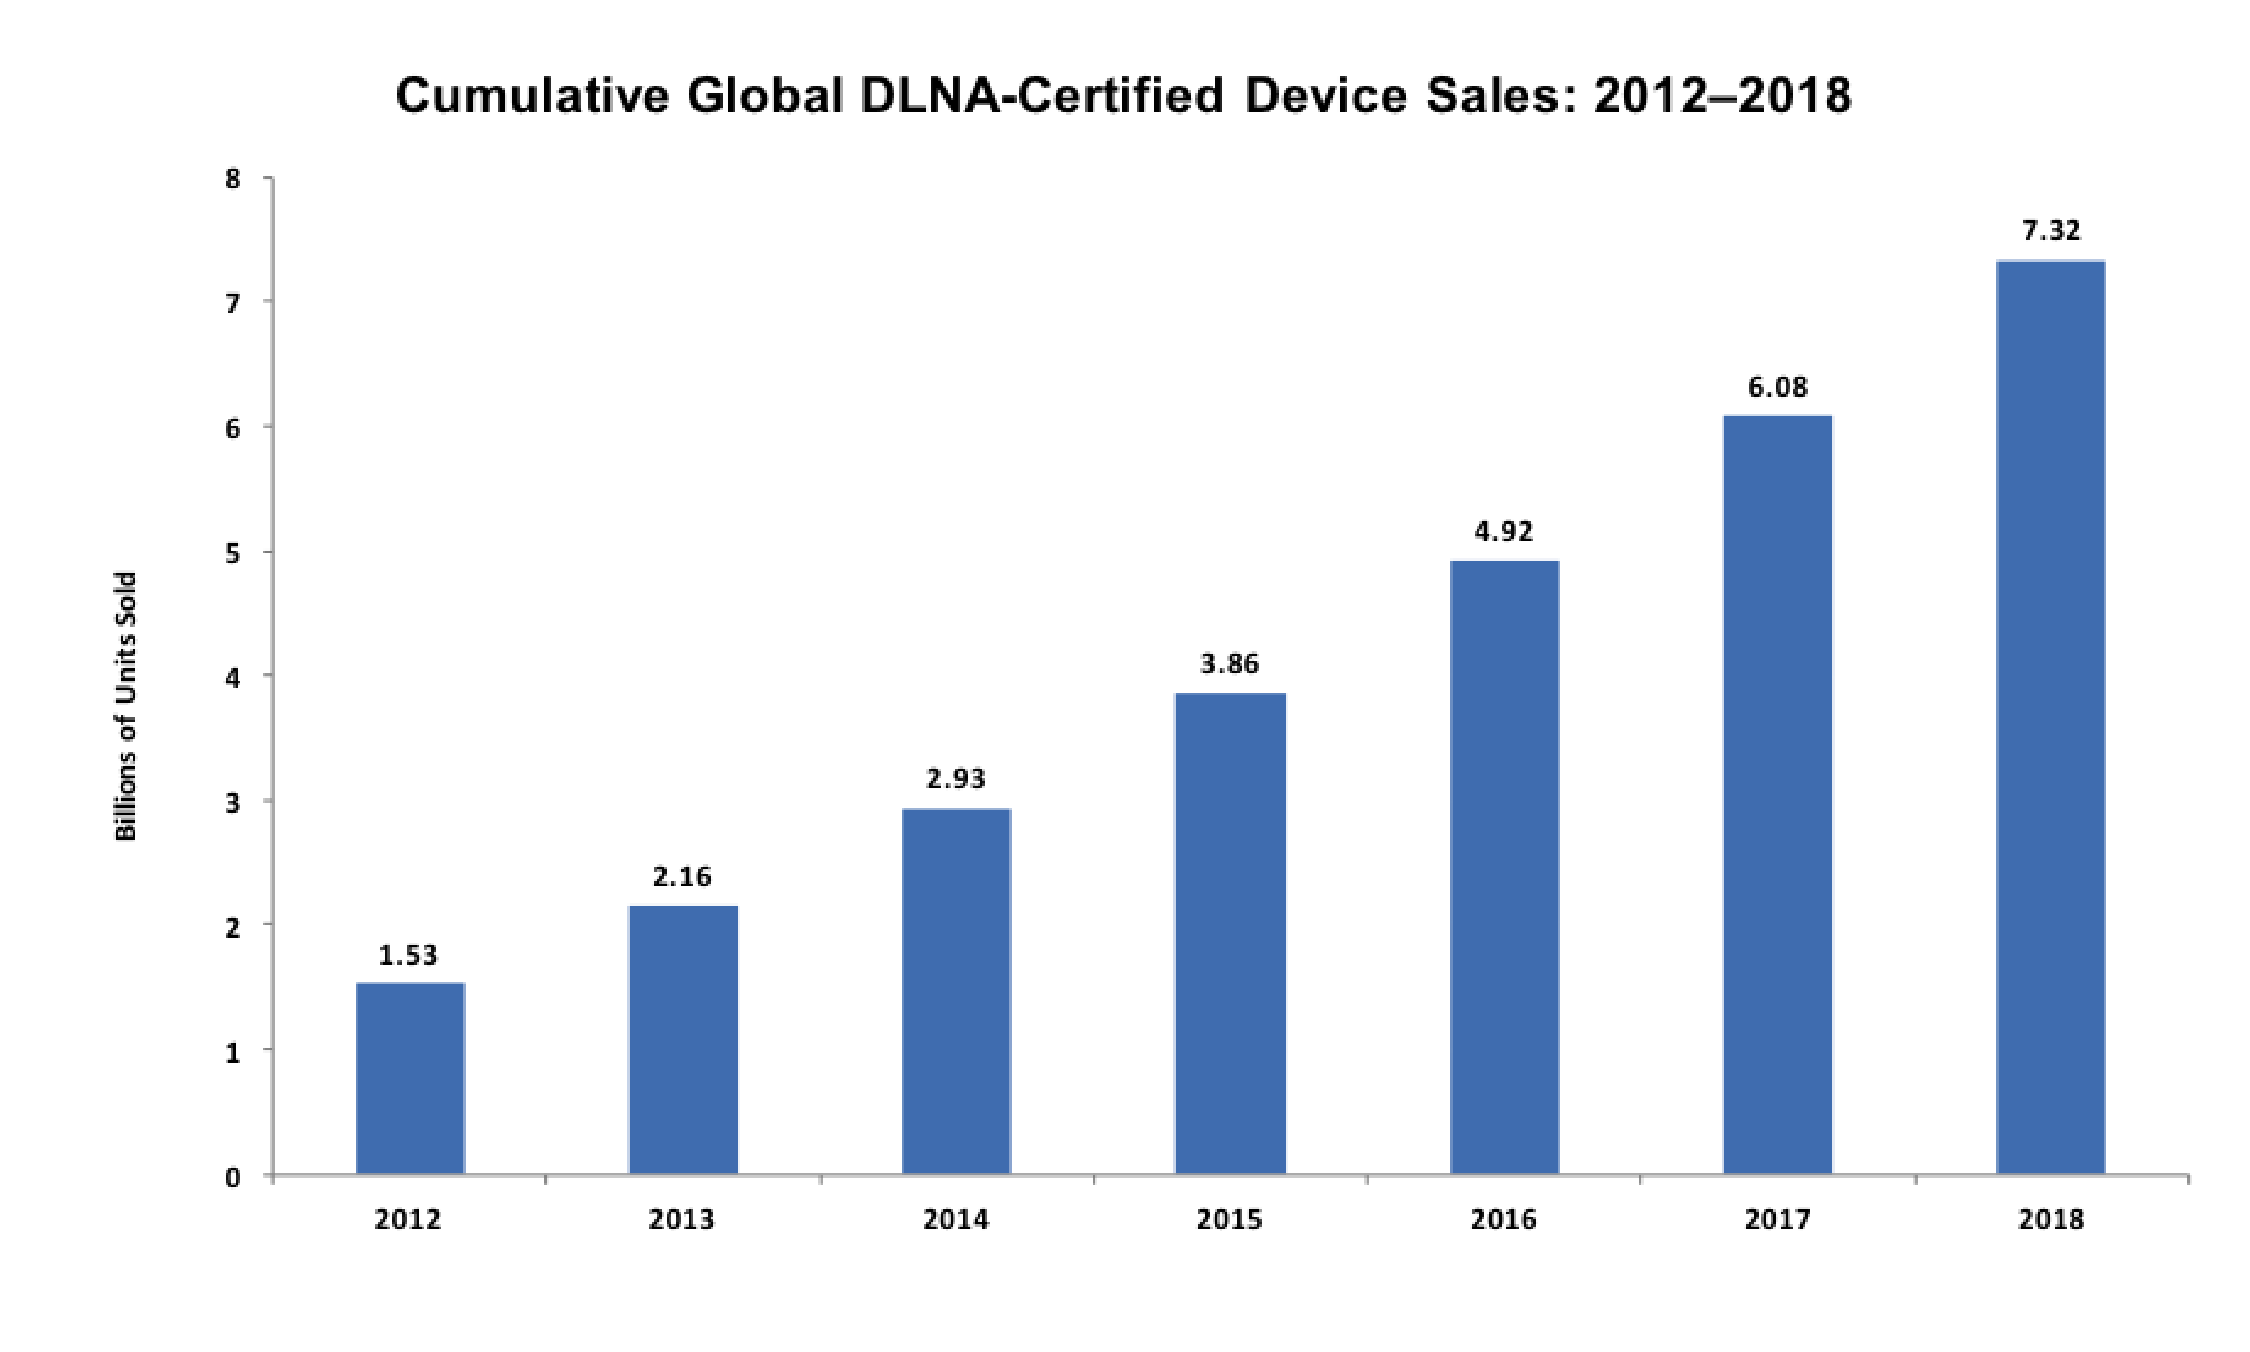
\includegraphics[height=9cm]{charts/dlna_market}
\caption{Cumulative Global DLNA-Certified Device sales \label{dlna_market}}
\end{figure}

\item[--]Airplay is bundled with Apple products, with great sales of Apple TV, Airport Express, 
Mac, iPhone, iPad, iPod, many family has just use Apple's product for everything. Thus Airplay 
becomes the easiest way to build home networking solution, and maybe the only solution for those 
Apple users, since a lot of speaker manufactures implement their own Airplay receiver on their 
Airplay compatible speakers. And indeed it provides enough easy to use features to fulfill daily usage.
\item[--]Since bundled with Android operating system, Miracast has experienced a fast growth in 
the past two years, many TVs built in the Miracast support to accept peer-to-peer Wi-Fi direct connection.
\item[--]Chromecast dongle is really cheap device that everyone wants to try, it can easily upgrade 
old TV to "Smart TV", and since Google has provided good content support for it, it is soon accepted 
by huge amount of users. Except for Google play online sales, it also ranked top 3 best selling devices 
recently.
\end{itemize}

\subsubsection{Technology feature}
\begin{enumerate}
\item Meida format support \\
Airplay and Chromecast has very limited media format support since they are only limited device 
types, so far Chromecast has only 1 device released. Apple TV now has 3rd generation box, but the 
media format support has not changed so much, the main improvement is the 1080p high resolution 
video support. On the other hand, DLNA has specified mandatory media formats in its specification, 
the "must have" formats only include MP3 and LPCM for music, JPEG for images and MP4 for video. 
Since Miracast is a screen mirroring technology, all formats can be played on device can be streamed.

\item Networking technologies used \\

A short technology specification comparison is made to help better understanding
the existing solutions, table \ref{Table1} below shows the main technology used
for different popular solutions.
%% table 1, compare technology
\begin{table}[htb]
\caption{Technology used \label{Table1}}
\begin{center}
\fbox{
\begin{tabular}{c|l|l|l}  
\textbf{ } & Device discovery & Control Protocol & Streaming protocol \\ \hline
\textbf{DLNA} & SSDP & UPnP & HTTP \\ \hline
\textbf{AirPlay} & Multicast DNS & HTTP & HTTP/RTSP \\ \hline
\textbf{Chromecast} & DIAL & Chromecast & HTTP \\ \hline
\textbf{Miracast} & Wi-Fi direct &  & Wi-Fi direct
\end{tabular}
}
\end{center}
\end{table}

Apart from those basic technological details, some standards also offer advanced
features compared to other solutions. For example, screen mirroring is an
interesting feature that many standards offers. Table \ref{Table2} below shows
what advanced features each standard provides.
%% table 2, compare advance feature
\begin{table}[htb]
\caption{Advanced feature comparison \label{Table2}}
\begin{center}
\fbox{
\begin{tabular}{c|l|l|l|l}  
\textbf{ } & DLNA & AirPlay & Chromecast & Miracast \\ \hline
\textbf{Screen mirroring} & No & Yes & No & Yes \\ \hline
\textbf{Multiple connection} & Yes & No & No & No \\ \hline
\textbf{Authentication} & No & Yes & No & Yes
\end{tabular}
}
\end{center}
\end{table}


\end{enumerate} 

According to the comparison, each standard have its own features and uses different protocols 
to communicate. But there are common features supported by most standards, such as HTTP media 
server is used quite much to handle video and photo streaming. UPnP device discovery protocol 
SSDP is used quite a lot for device discovery. 

Since there is some similarity that is used by most standards, there is possibility to make 
some application that include all these standard architecture and work with those protocols. 
Making an Android application to connect those devices becomes a doable work.

